\documentclass[aspectratio=169,10pt]{beamer}
\usetheme[progressbar=frametitle,numbering=fraction,block=fill]{metropolis}
\usepackage{booktabs,amsmath,tabularx,multicol}
\usepackage{tikz}
\usepackage[siunitx]{circuitikz}
\usetikzlibrary{arrows.meta,positioning,calc}
\definecolor{kth}{RGB}{25,84,166}
\definecolor{kthl}{RGB}{98,152,210}
\definecolor{hs}{RGB}{200,70,50}
\definecolor{ls}{RGB}{50,100,190}
\definecolor{pri}{RGB}{60,140,80}
\setbeamercolor{frametitle}{bg=kth,fg=white}
\setbeamercolor{progress bar}{fg=kthl,bg=kth!20}
\setbeamercolor{title separator}{fg=kthl}
\setbeamercolor{alerted text}{fg=hs}
\graphicspath{{figs/}{../paper/figures/}{../gate-bump/figures/}{../gate-driver/figures/}{../pcb-fab/figures/}{../design-report-v2/figures/}}
\newcommand{\src}[1]{\vfill{\tiny\color{gray}#1}}

\title{GaN Building Block for a 1200\,V, 150\,kW Stacked Polyphase Bridge Inverter}
\subtitle{Design procedure, gate drive, layout and the Rev A fabrication board}
\author{Enes Ayaz}
\institute{KTH Royal Institute of Technology}
\date{October 2026}

\begin{document}
\maketitle

\begin{frame}{Outline}
\begin{multicols}{2}
\begin{enumerate}
\item System and specification
\item Voltage class and transistor
\item Layout and gate-drive concept
\item Number of devices in parallel
\item DC link
\item Parasitics, switching, losses, thermal
\item Gate bump and negative bias
\item Gate-driver selection and scaling
\item Integration and machine side
\item Rev A fabrication board
\item Measurements and bring-up
\item Status and next steps
\end{enumerate}
\end{multicols}
\end{frame}

%==================================================================== 1
\section{System and specification}
\begin{frame}{Stacked polyphase bridge (SPB) inverter}
\begin{columns}[T]
\column{0.58\textwidth}
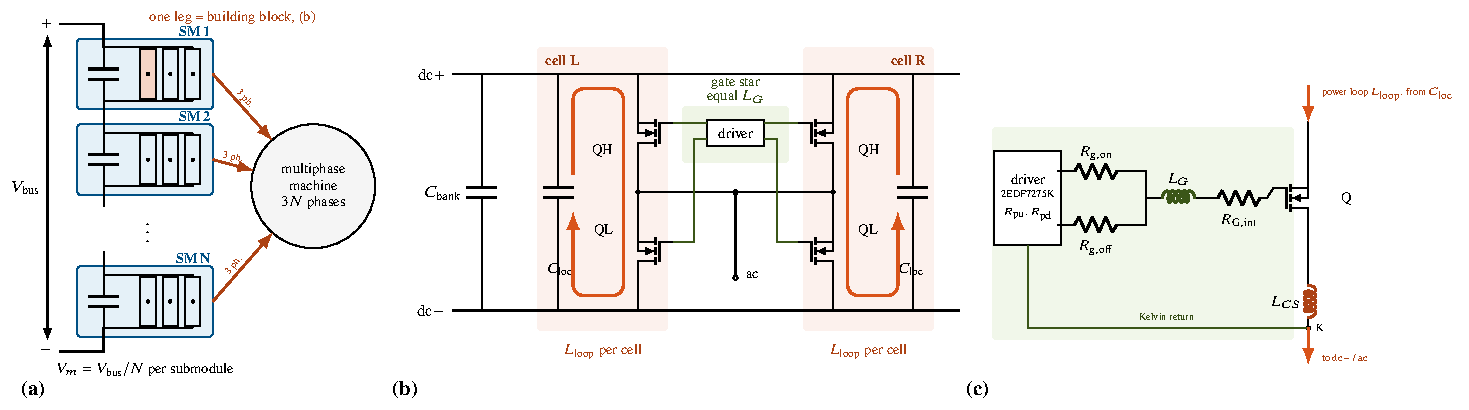
\includegraphics[width=\linewidth]{fig_spb_standalone.pdf}
\column{0.40\textwidth}
\begin{itemize}\small
\item 1200\,V bus, 150\,kW traction inverter
\item $N$ three-phase submodules in series on the DC side, each feeding one winding set of a multiphase machine
\item $V_m = V_\mathrm{bus}/N$: the transistor voltage class becomes a \alert{design variable}
\item Phase current set by power and bus voltage: $\approx$\,100\,A$_\mathrm{rms}$ (M\,=\,1.15)
\item Chosen: $N=16$, $V_m=75$\,V, 3\,kW per leg, 9\,kW per submodule
\end{itemize}
\end{columns}
\end{frame}

\begin{frame}{Design procedure}
\centering
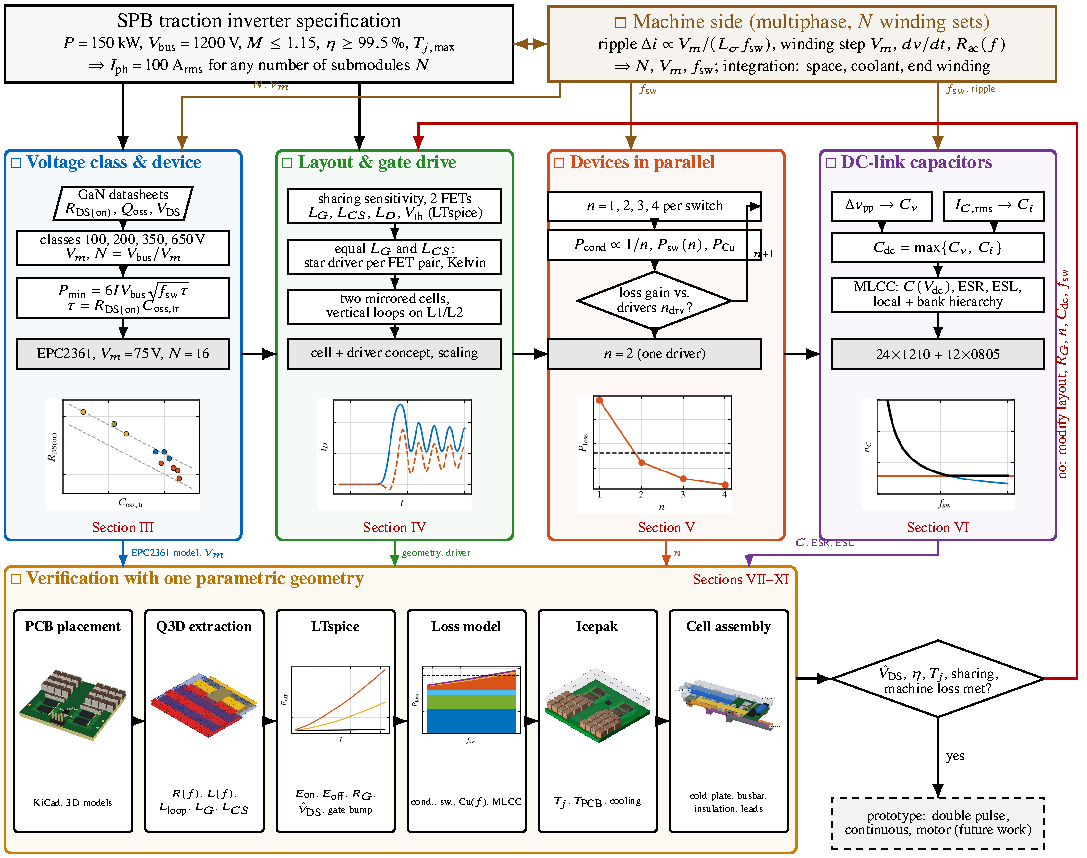
\includegraphics[width=0.92\linewidth,height=0.78\textheight,keepaspectratio]{fig_flow_standalone.pdf}
\small Specification $\rightarrow$ voltage class $\rightarrow$ layout / gate drive $\rightarrow$ number of parallel devices $\rightarrow$ DC link $\rightarrow$ verification, with the machine side feeding back $N$ and $f_\mathrm{sw}$.
\end{frame}

%==================================================================== 2
\section{Voltage class and transistor}
\begin{frame}{Voltage class: why 100\,V GaN}
\begin{columns}[T]
\column{0.6\textwidth}
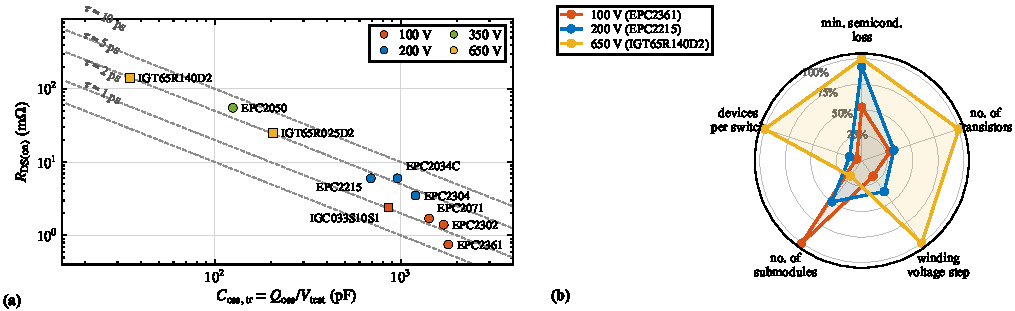
\includegraphics[width=\linewidth]{fig_devices.pdf}
\column{0.38\textwidth}
\small
\begin{itemize}
\item At fixed bus voltage and phase current the minimum semiconductor loss scales with the device time constant $R_\mathrm{DS(on)}C_\mathrm{oss,tr}$
\item 100\,V GaN gives the lowest product among 100--650\,V Si/SiC/GaN candidates
\item Selected: \textbf{EPC2361}, 100\,V, 0.75\,m$\Omega$ typ, 3\,$\times$\,5\,mm, top-side cooling
\end{itemize}
\end{columns}
\end{frame}

\begin{frame}{EPC2361 key data}
\begin{columns}[T]
\column{0.55\textwidth}
\small
\begin{tabular}{@{}ll@{}}
\toprule
$V_\mathrm{DS}$ / transient & 100 / 120\,V \\
$R_\mathrm{DS(on)}$ & 0.75\,m$\Omega$ typ (1.0 max) \\
$V_\mathrm{GS}$ range & $-4$ \dots\ $+6$\,V \\
$V_\mathrm{GS(th)}$ & 0.8 / 1.1 / 2.5\,V \\
$C_\mathrm{iss}$ / $C_\mathrm{oss}$ / $C_\mathrm{rss}$ & 3599 / 1019 / 13\,pF \\
$Q_G$ / $Q_{GD}$ / $Q_\mathrm{OSS}$ & 28 / 3.8 / 90\,nC \\
$R_\mathrm{G,int}$ & 0.4\,$\Omega$ \\
$R_{\theta\mathrm{JC}}$ top / $R_{\theta\mathrm{JB}}$ & 0.2 / 1.5\,K/W \\
\bottomrule
\end{tabular}
\column{0.43\textwidth}
\small
\begin{itemize}
\item Low threshold and $-4$\,V limit: gate drive needs care (bump, negative bias)
\item Top of the package at \alert{source potential}: thermal interface must insulate
\item Seven interleaved stripes, pad 2 next to the gate is the natural Kelvin point
\end{itemize}
\end{columns}
\end{frame}

\begin{frame}{Voltage utilisation: 75\,V or 60\,V submodules}
\begin{columns}[T]
\column{0.58\textwidth}
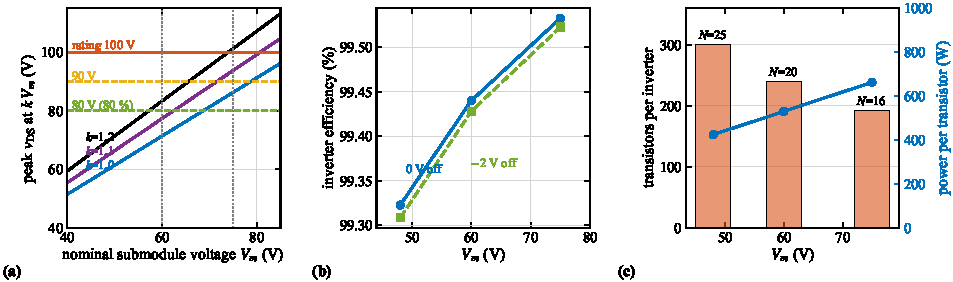
\includegraphics[width=\linewidth]{utilization.pdf}
\column{0.4\textwidth}
\small
\begin{itemize}
\item 75\,V nominal with $k=1.2$ overshoot/ripple factor $\Rightarrow$ $\approx$\,100\,V peak at the device
\item Keeping $\leq 80$\,V needs $V_m \leq 57$\,V ($k=1.2$) or $\leq 69$\,V ($k=1$)
\item Trade-off: 60\,V submodules $\rightarrow$ $N=20$, more cells and drivers, more margin
\item Rev A board designed and tested for 75\,V
\end{itemize}
\end{columns}
\end{frame}

%==================================================================== 3
\section{Layout and gate-drive concept}
\begin{frame}{Building block layout: two mirrored cells, centre driver}
\begin{columns}[T]
\column{0.5\textwidth}
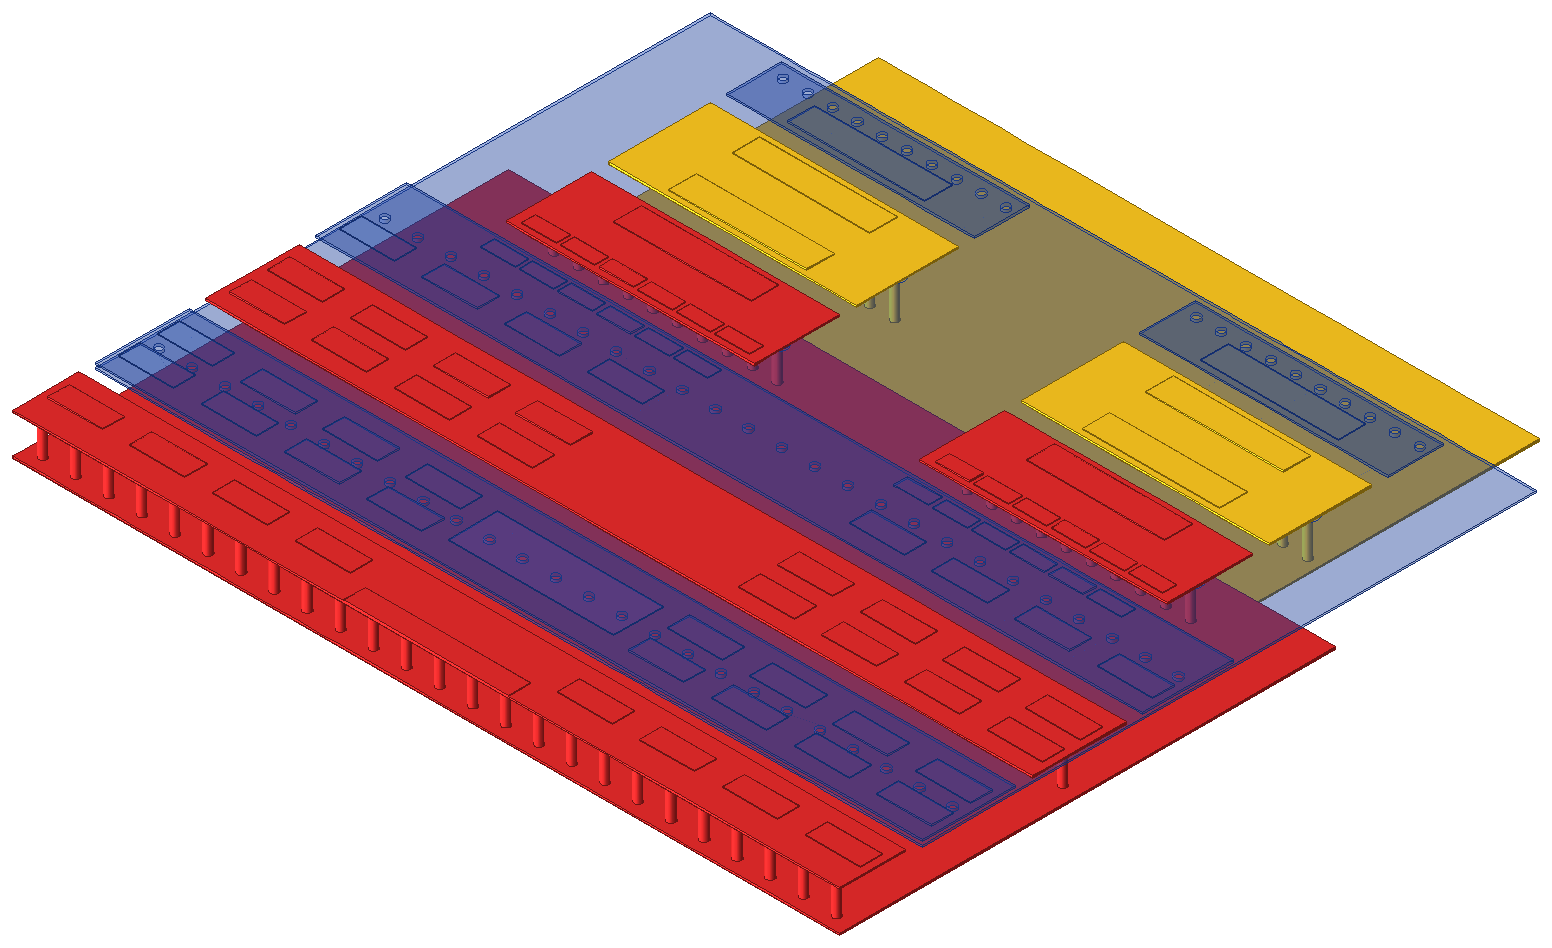
\includegraphics[width=\linewidth]{q3d_model.png}
\column{0.48\textwidth}
\small
\begin{itemize}
\item One half-bridge leg, 2\,$\times$\,EPC2361 per switch in \textbf{two mirrored commutation cells}
\item Vertical power loop: L1 forward, L2 (DC$-$) return 0.1\,mm below $\Rightarrow$ flux cancellation
\item Local 0805 MLCCs at the drains, 1210 bank above both cells
\item Driver on the symmetry line: identical gate loops to both transistors
\item Q3D: $L_\mathrm{loop} = 0.374$\,nH per cell (copper + MLCC ESL)
\end{itemize}
\end{columns}
\end{frame}

\begin{frame}{Why symmetry: current-sharing sensitivity}
\begin{columns}[T]
\column{0.6\textwidth}
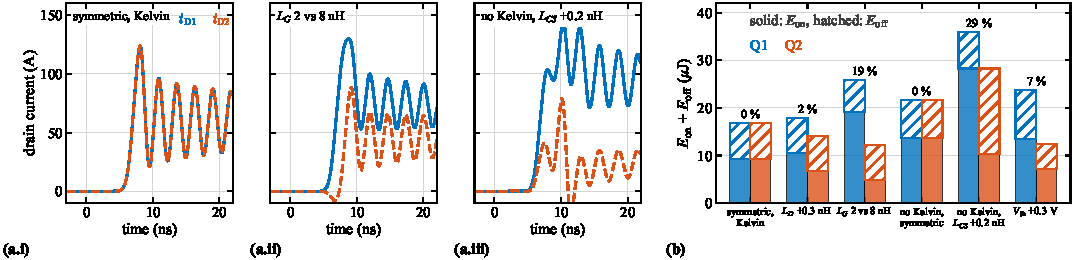
\includegraphics[width=\linewidth]{fig_sharing.pdf}
\column{0.38\textwidth}
\small
\begin{itemize}
\item Static sharing is fine ($R_\mathrm{DS(on)}$ has positive TC)
\item Dynamic sharing is set by the gate circuits:
\begin{itemize}\footnotesize
\item gate-loop mismatch 2 vs 8\,nH $\rightarrow$ 19\,\% imbalance, 4:1 $E_\mathrm{on}$
\item common-source mismatch without Kelvin $\rightarrow$ 29\,\%, $2.8\times E_\mathrm{on}$ in one device
\end{itemize}
\item $\Rightarrow$ star-connected gate drive with Kelvin returns, one driver channel per pair
\end{itemize}
\end{columns}
\end{frame}

\begin{frame}{Kelvin source on the EPC2361}
\begin{columns}[T]
\column{0.52\textwidth}
\centering
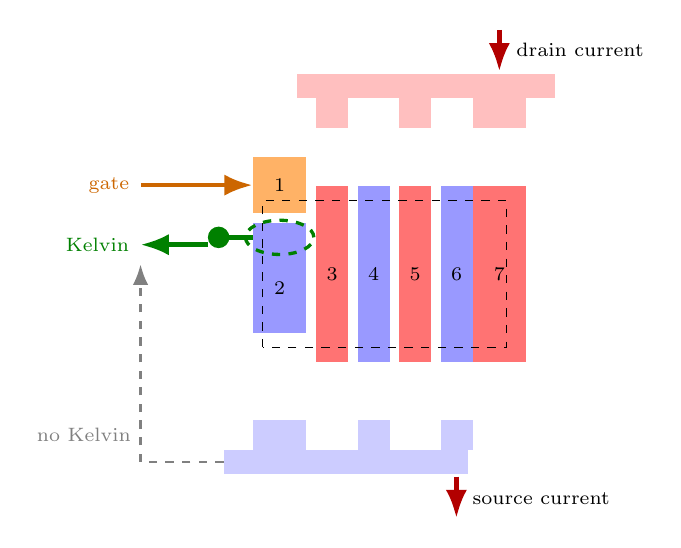
\begin{tikzpicture}[scale=0.62]
% drain / source copper
\fill[red!25] (1.0,3.6) rectangle (6.3,4.1);
\foreach \x/\w in {1.725/0.65,3.425/0.65,5.152/1.10} \fill[red!25] (\x-\w/2,3.0) rectangle (\x+\w/2,3.6);
\fill[blue!20] (-0.5,-4.1) rectangle (4.5,-3.6);
\foreach \x/\w in {0.648/1.10,2.575/0.65,4.275/0.65} \fill[blue!20] (\x-\w/2,-3.6) rectangle (\x+\w/2,-3.0);
% pads
\fill[orange!60] (0.097,1.25) rectangle (1.199,2.39);
\fill[blue!40] (0.097,-1.21) rectangle (1.199,1.05);
\foreach \x in {1.725,3.425} \fill[red!55] (\x-0.325,-1.8) rectangle (\x+0.325,1.8);
\foreach \x in {2.575,4.275} \fill[blue!40] (\x-0.325,-1.8) rectangle (\x+0.325,1.8);
\fill[red!55] (4.601,-1.8) rectangle (5.703,1.8);
\draw[dashed] (0.3,-1.5) rectangle (5.3,1.5);
\node at (0.65,1.82) {\scriptsize 1};
\node at (0.65,-0.3) {\scriptsize 2};
\foreach \x/\n in {1.725/3,2.575/4,3.425/5,4.275/6,5.152/7} \node at (\x,0) {\scriptsize \n};
% Kelvin
\draw[green!50!black,line width=1.2pt,dashed] (0.65,0.75) ellipse (0.7 and 0.35);
\fill[green!50!black] (-0.6,0.75) circle (0.22);
\draw[green!50!black,line width=1.6pt] (0.097,0.75) -- (-0.38,0.75);
\draw[green!50!black,line width=1.6pt,-{Latex}] (-0.82,0.6) -- (-2.2,0.6) node[left]{\scriptsize Kelvin};
\draw[orange!80!black,line width=1.6pt,{Latex}-] (0.097,1.82) -- (-2.2,1.82) node[left]{\scriptsize gate};
\draw[gray,line width=1pt,dashed,-{Latex}] (-0.5,-3.85) -- (-2.2,-3.85) -- (-2.2,0.2);
\node[gray,left] at (-2.2,-3.3) {\scriptsize no Kelvin};
\draw[red!70!black,line width=1.6pt,-{Latex}] (5.15,5.0) -- (5.15,4.15);
\draw[red!70!black,line width=1.6pt,-{Latex}] (4.27,-4.15) -- (4.27,-5.0);
\node[right] at (5.3,4.6) {\scriptsize drain current};
\node[right] at (4.4,-4.6) {\scriptsize source current};
\end{tikzpicture}
\column{0.46\textwidth}
\small
\begin{itemize}
\item Pad 2 is a separate source pad next to the gate pad; its gate end carries almost no load current
\item Kelvin via at that end; return routed to the driver on its own path (L2 / L4)
\item Gate loop (horizontal) $\perp$ power loop (vertical): minimum coupling
\item Q3D: $L_{CS}$ = \textbf{0.030\,nH} with Kelvin, 0.061\,nH without $\Rightarrow$ $\approx$\,0.5 vs 1.0\,V subtracted from $V_{GS}$ at 17\,A/ns
\end{itemize}
\end{columns}
\end{frame}

%==================================================================== 4
\section{Number of devices in parallel}
\begin{frame}{How many EPC2361 per switch?}
\centering
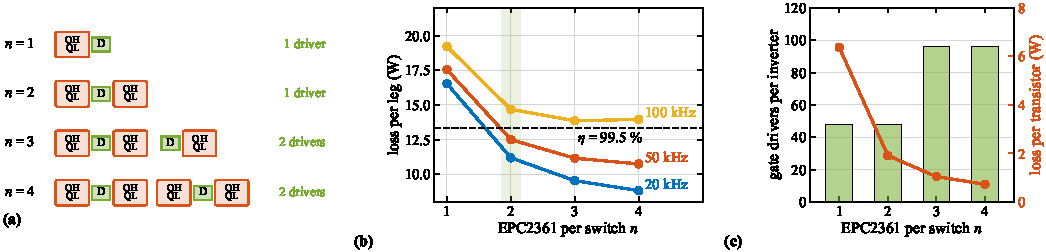
\includegraphics[width=\linewidth,height=0.62\textheight,keepaspectratio]{fig_npar.pdf}
\small
\begin{itemize}
\item 1 $\rightarrow$ 2 devices: large drop in conduction loss and per-device loss
\item 3 or 4 devices: only $-1.3$ / $-1.7$\,W more, while output-charge loss grows and the drivers double (48 $\rightarrow$ 96)
\item \textbf{Two per switch}: two cells with one centre driver
\end{itemize}
\end{frame}

%==================================================================== 5
\section{DC link}
\begin{frame}{DC-link capacitors}
\begin{columns}[T]
\column{0.55\textwidth}
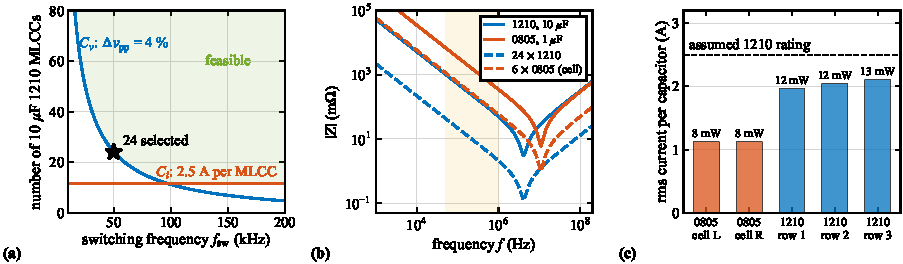
\includegraphics[width=\linewidth]{fig_dclink.pdf}
\column{0.43\textwidth}
\scriptsize
\begin{tabular}{@{}lcc@{}}
\toprule
 & local & bank \\
\midrule
Part & TDK 0805 & Murata 1210 \\
 & 1\,\textmu F 100\,V X7S & 10\,\textmu F 100\,V X7S \\
Number per leg & 2\,$\times$\,6 & 24 \\
$C_\mathrm{eff}$ at 75\,V & 0.45\,\textmu F & 3.0\,\textmu F \\
ESR / ESL & 6\,m$\Omega$ / 0.48\,nH & 3\,m$\Omega$ / 0.5\,nH \\
Ripple per part & 1.1\,A$_\mathrm{rms}$ & 2.0--2.1\,A$_\mathrm{rms}$ \\
Loss per part & 7.5\,mW & 11.5--13.3\,mW \\
\bottomrule
\end{tabular}

\small
\begin{itemize}
\item Bank sized by voltage ripple below $\approx$\,50\,kHz, by ripple current above
\item Total capacitor loss $\approx$\,0.39\,W per leg
\end{itemize}
\end{columns}
\end{frame}

%==================================================================== 6
\section{Parasitics, switching, losses, thermal}
\begin{frame}{Extracted parasitics (Q3D)}
\begin{columns}[T]
\column{0.45\textwidth}
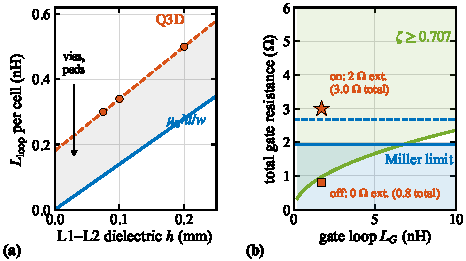
\includegraphics[width=\linewidth]{fig_parasitics.pdf}
\column{0.53\textwidth}
\small
\begin{tabular}{@{}lr@{}}
\toprule
Power loop per cell (copper + ESL) & 0.374\,nH \\
Gate loop $L_G$ per transistor & 1.71\,nH \\
$L_{CS}$, Kelvin / no Kelvin & 0.030 / 0.061\,nH \\
Gate loop -- gate loop mutual & 0.46\,nH \\
Busbar, leg to leg (1\,MHz) & 3.35\,nH \\
Busbar, series tab to leg & 41\,nH \\
\bottomrule
\end{tabular}
\vspace{1ex}

\footnotesize Busbar: DC$+$ and DC$-$ tabs leave at opposite ends (41\,nH); bring them out together or use a laminated cell interconnect.
\end{columns}
\end{frame}

\begin{frame}{Switching behaviour}
\centering
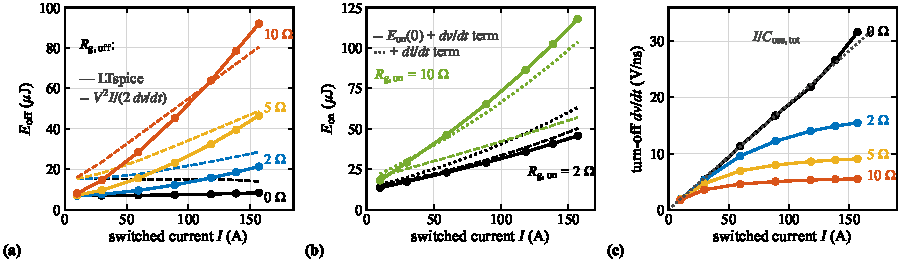
\includegraphics[width=\linewidth,height=0.72\textheight,keepaspectratio]{fig_switching.pdf}
\small LTspice with the Q3D power loop and gate star, 75\,V, $R_\mathrm{g,on}/R_\mathrm{g,off}$ = 2 / 0\,$\Omega$ external.
\end{frame}

\begin{frame}{Losses and efficiency}
\begin{columns}[T]
\column{0.6\textwidth}
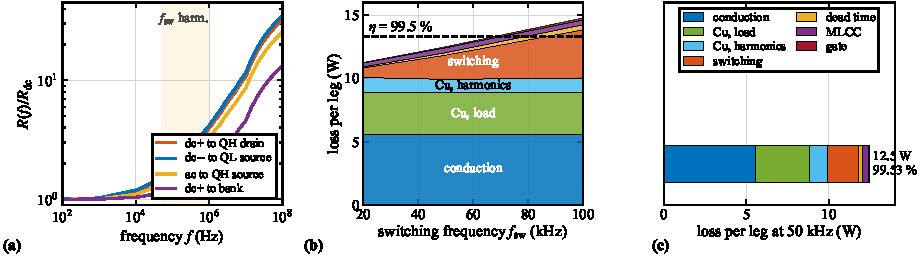
\includegraphics[width=\linewidth]{fig_losses.pdf}
\column{0.38\textwidth}
\small
\begin{itemize}
\item Rated point (75\,V, 100\,A$_\mathrm{rms}$, 50\,kHz): \textbf{12.5\,W per leg}, $\eta$ = 99.53\,\%
\item Worst case 14.3\,W (99.46\,\%)
\item 1.91\,W per transistor
\item Copper and switching harmonics add $\approx$\,1/3 to the DC copper loss
\end{itemize}
\end{columns}
\end{frame}

\begin{frame}{Thermal design}
\begin{columns}[T]
\column{0.6\textwidth}
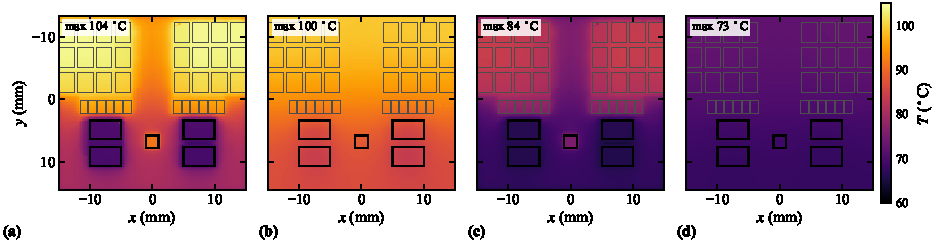
\includegraphics[width=\linewidth]{fig_thermal.pdf}
\column{0.38\textwidth}
\small
\begin{itemize}
\item Top-side cooling through an insulating interface to a liquid cold plate (integration concept)
\item Icepak: $T_j \approx 64\,^\circ$C at the rated point
\item Lab: fan heatsink on the Rev A board (later slide)
\end{itemize}
\end{columns}
\end{frame}

%==================================================================== 7
\section{Gate bump and negative bias}
\begin{frame}{Gate bump at the high side}
\begin{columns}[T]
\column{0.58\textwidth}
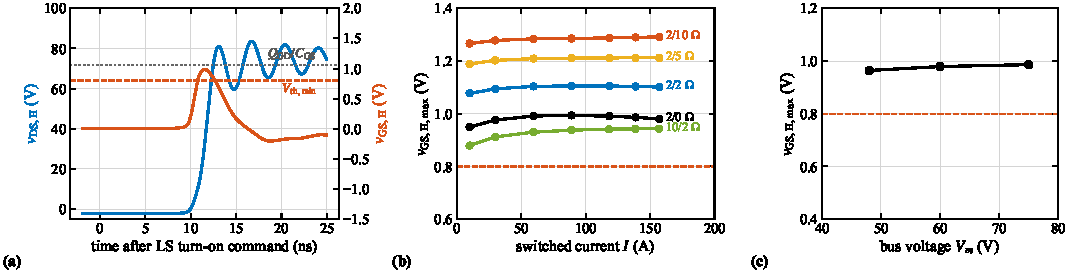
\includegraphics[width=\linewidth]{bump_mechanism.pdf}
\column{0.4\textwidth}
\small
\begin{itemize}
\item When the low side turns on, the high-side drain sees $dv/dt$: Miller charge flows into $C_{GS}$
\item Bump $\approx Q_{GD}/C_{GS} \approx 1.06$\,V, $\approx$\,2\,ns, \textbf{independent of current and voltage}
\item Below the 1.1\,V typical threshold, close to the 0.8\,V minimum: no shoot-through in simulation, but little margin
\end{itemize}
\end{columns}
\end{frame}

\begin{frame}{Mitigation: negative off-voltage}
\begin{columns}[T]
\column{0.58\textwidth}
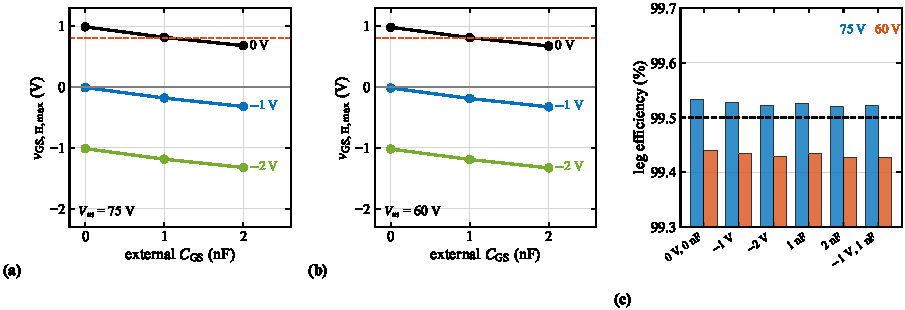
\includegraphics[width=\linewidth]{bump_mitigation.pdf}
\column{0.4\textwidth}
\small
\begin{itemize}
\item With $-1$\,V off-voltage the peak falls from 0.99\,V to $-0.01$\,V
\item Undershoot $-2.3$\,V, rating $-4$\,V
\item Cost: reverse conduction drop in the dead time rises by 1\,V
\item Dead-time loss 0.20 / 0.29 / 0.38\,W per leg for 0 / $-1$ / $-2$\,V
\item \textbf{Chosen: $\approx -1.24$\,V}
\end{itemize}
\end{columns}
\end{frame}

%==================================================================== 8
\section{Gate-driver selection and scaling}
\begin{frame}{Driver: Infineon 2EDF7275K}
\begin{columns}[T]
\column{0.58\textwidth}
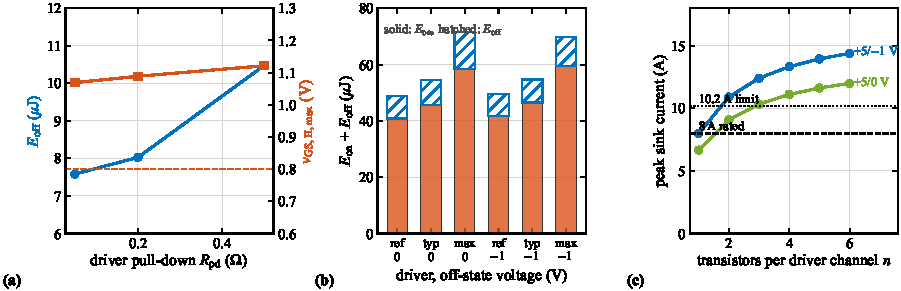
\includegraphics[width=\linewidth]{drv_output_stage.pdf}
\column{0.4\textwidth}
\small
\begin{itemize}
\item Dual isolated channel, 4\,A source / 8\,A sink, 0.85 / 0.35\,$\Omega$
\item 4\,V UVLO: allows a split $+5/-1.24$\,V supply per channel
\item Sink strength sets the turn-off ($E_\mathrm{off}$), not the bump
\item LGA-13, 5\,$\times$\,5\,mm; functional isolation only
\end{itemize}
\end{columns}
\end{frame}

\begin{frame}{Negative rail vs dead-time loss}
\centering
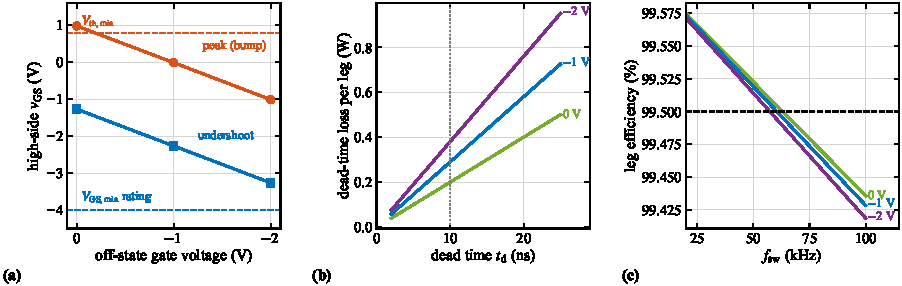
\includegraphics[width=\linewidth,height=0.75\textheight,keepaspectratio]{drv_negative_rail.pdf}
\end{frame}

\begin{frame}{More parallel devices need more drivers}
\begin{columns}[T]
\column{0.58\textwidth}
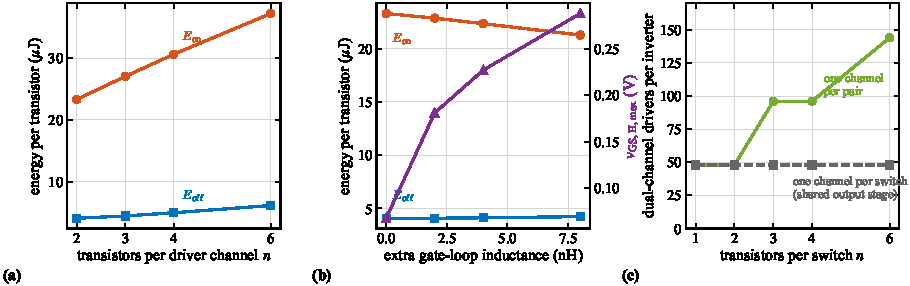
\includegraphics[width=\linewidth]{drv_scaling.pdf}
\column{0.4\textwidth}
\small
\begin{itemize}
\item One channel drives two transistors symmetrically
\item Sharing one channel among 3 / 4 / 6 transistors: $E_\mathrm{on}$ per transistor $+16$ / $+31$ / $+60$\,\%
\item Peak sink current 12--14\,A, above the rating
\item Longer gate tree brings the bump back
\item $\Rightarrow$ scale in \textbf{pairs}, one channel per pair
\end{itemize}
\end{columns}
\end{frame}

%==================================================================== 9
\section{Integration and machine side}
\begin{frame}{Machine-integrated drive concept}
\begin{columns}[T]
\column{0.55\textwidth}
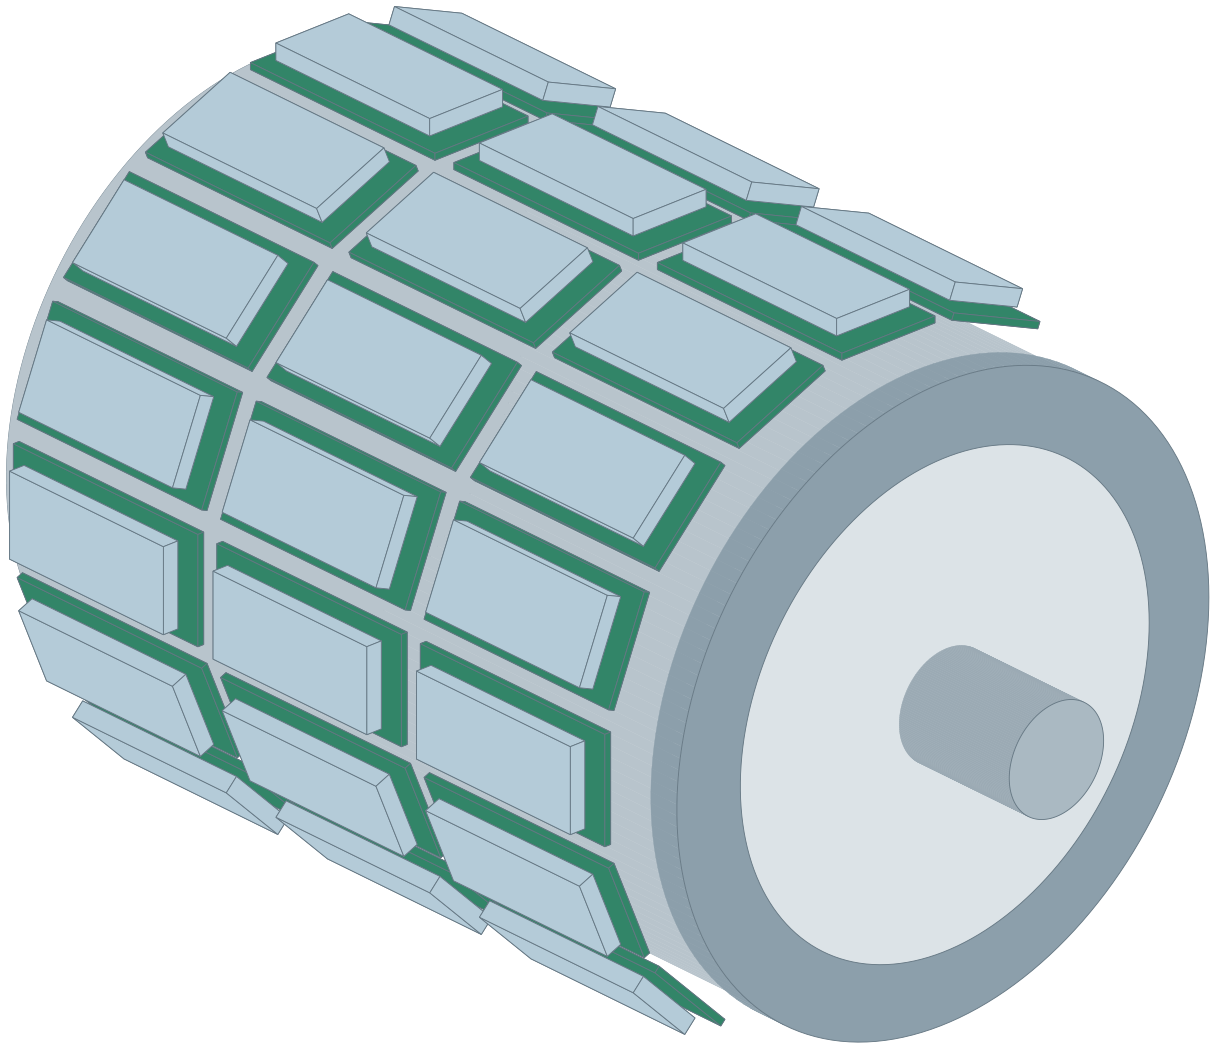
\includegraphics[width=\linewidth]{motor_integration.png}
\column{0.43\textwidth}
\small
\begin{itemize}
\item One submodule = one cell assembly on a liquid cold plate (AlN insulation)
\item Laminated busbar along the cells, phase leads to the winding sets
\item Machine side feeds back into $N$ (winding sets) and $f_\mathrm{sw}$ (ripple, iron loss)
\end{itemize}
\end{columns}
\end{frame}

\begin{frame}{Cell assembly and busbar}
\begin{columns}[T]
\column{0.5\textwidth}
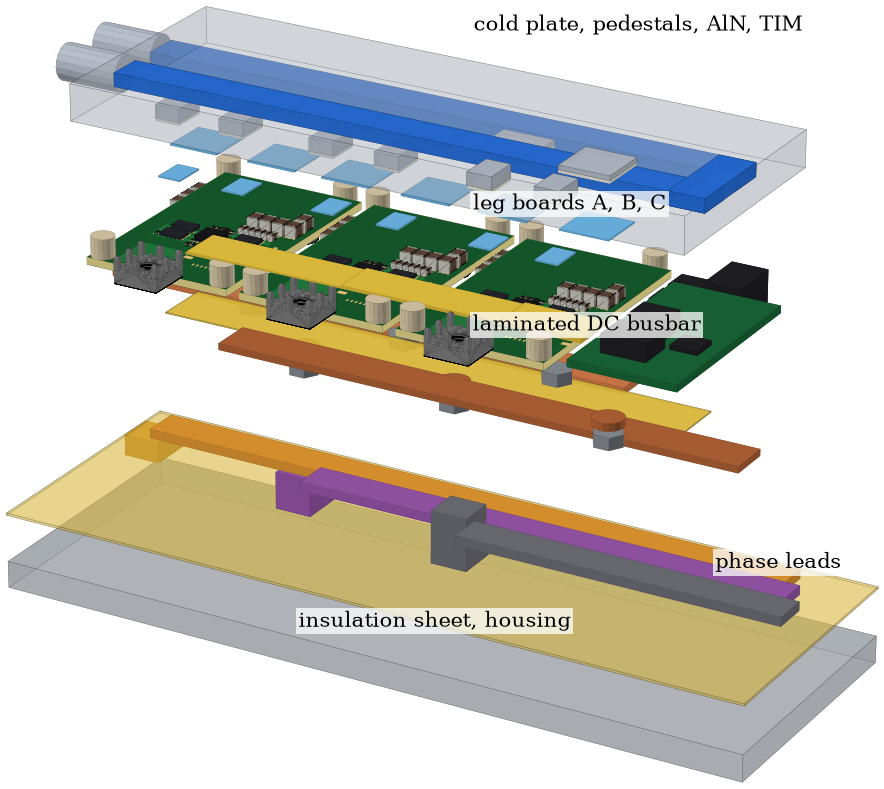
\includegraphics[width=\linewidth]{cell_exploded.png}
\column{0.48\textwidth}
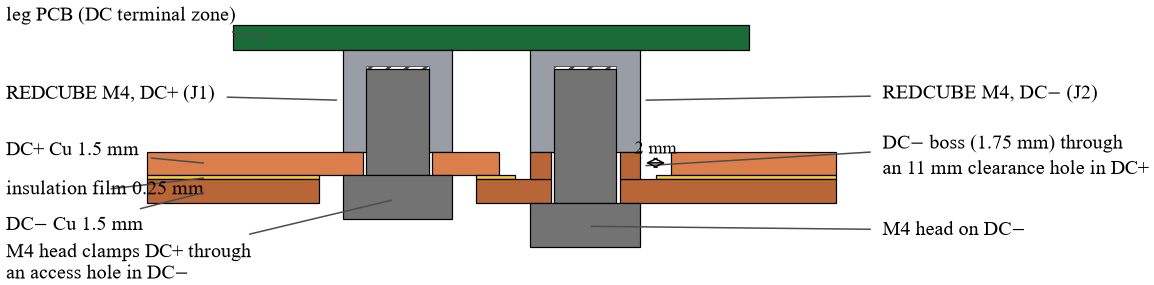
\includegraphics[width=\linewidth]{busbar_section.png}
\small
\begin{itemize}
\item Leg-to-leg busbar inductance 3.35\,nH (Q3D)
\item Series tabs: 41\,nH because DC$+$ and DC$-$ leave at opposite ends
\end{itemize}
\end{columns}
\end{frame}

%==================================================================== 10
\section{Rev A fabrication board}
\begin{frame}{Rev A board: overview}
\begin{columns}[T]
\column{0.6\textwidth}
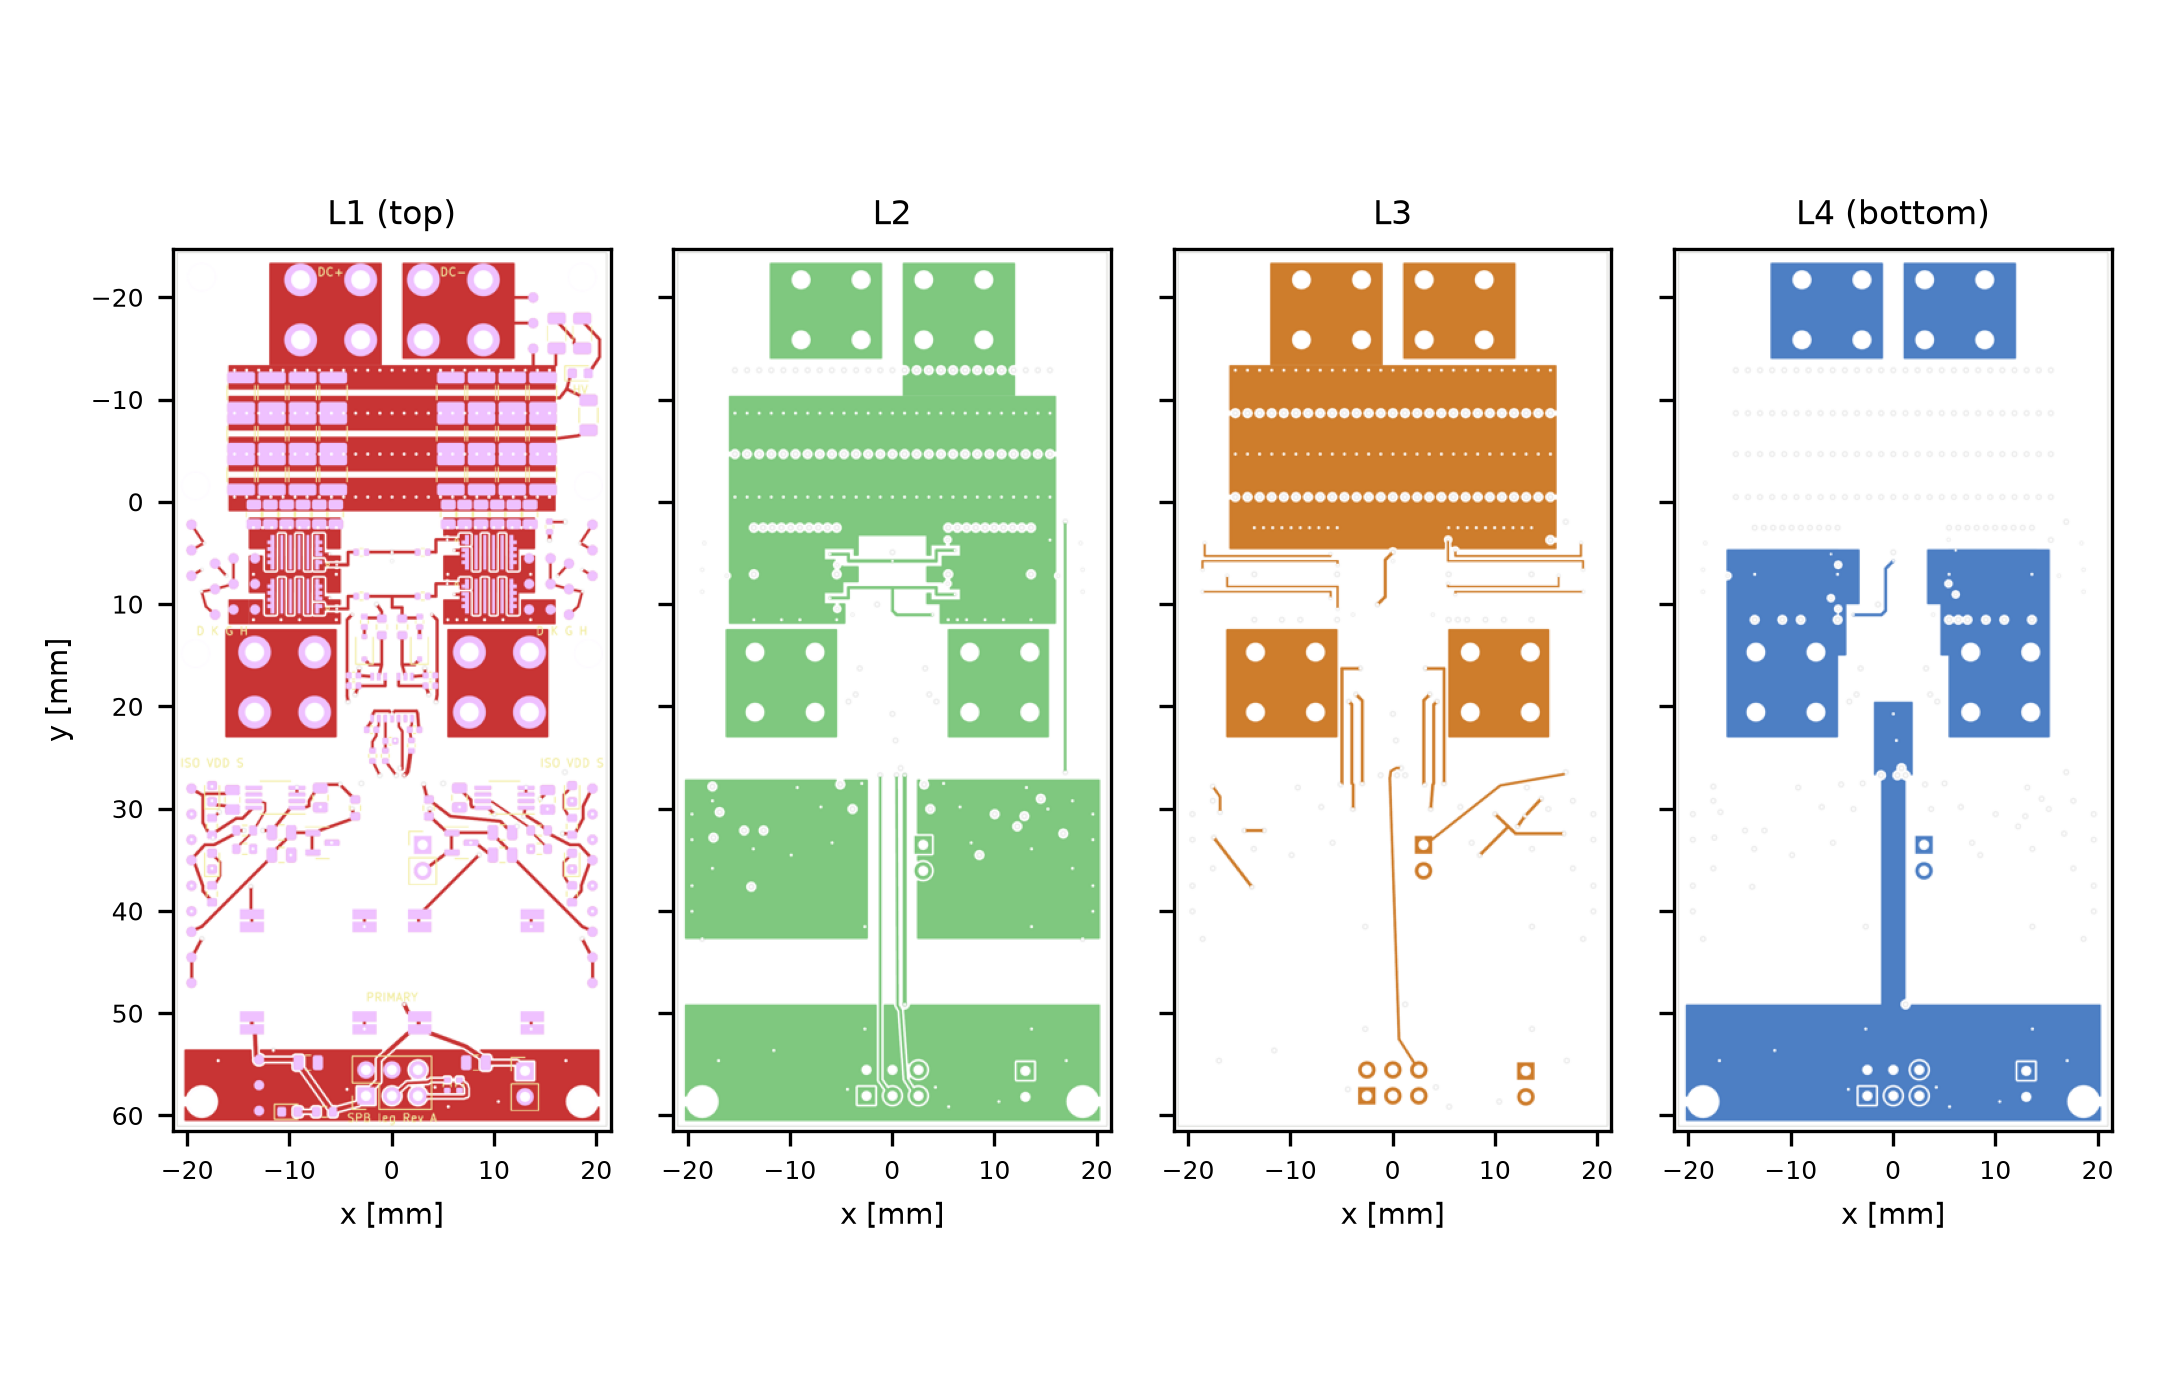
\includegraphics[width=\linewidth]{fig_layers.png}
\column{0.38\textwidth}
\small
\begin{itemize}
\item 42\,$\times$\,85.4\,mm, 4 layers, 4\,$\times$\,70\,\textmu m
\item DC terminals (top), two cells, driver corridor, AC terminals below each switch node, gate supplies, primary side (bottom)
\item Outer strips: heatsink holes, probe landings, LEDs
\item Fully scripted (KiCad~7 Python), DRC 0 / 0, wired schematic identical netlist
\end{itemize}
\end{columns}
\end{frame}

\begin{frame}{Stack-up and design rules}
\small
\begin{tabularx}{\linewidth}{@{}llX@{}}
\toprule
L1 70\,\textmu m & power, pads, gate stars & all components \\
prepreg 0.1\,mm & & vertical commutation loop \\
L2 70\,\textmu m & DC$-$ plane & loop return, Kelvin collectors in narrow keepouts \\
core $\approx$\,1.1\,mm & & \\
L3 70\,\textmu m & DC$+$ plane & HS gate trunk, supply columns, probe sense pairs \\
prepreg 0.1\,mm & & HS gate trunk over its Kelvin return \\
L4 70\,\textmu m & AC plane & switch node to J3/J4, HS Kelvin return, primary ground \\
\midrule
Rules & 0.15/0.15\,mm & power gaps 0.2\,mm under solder mask (IPC-2221B B4: 0.13\,mm for 51--100\,V) \\
Vias & 0.6/0.3\,mm, 0.45/0.25\,mm & no via-in-pad, standard process \\
\bottomrule
\end{tabularx}
\end{frame}

\begin{frame}{Gate loops in the driver corridor}
\centering
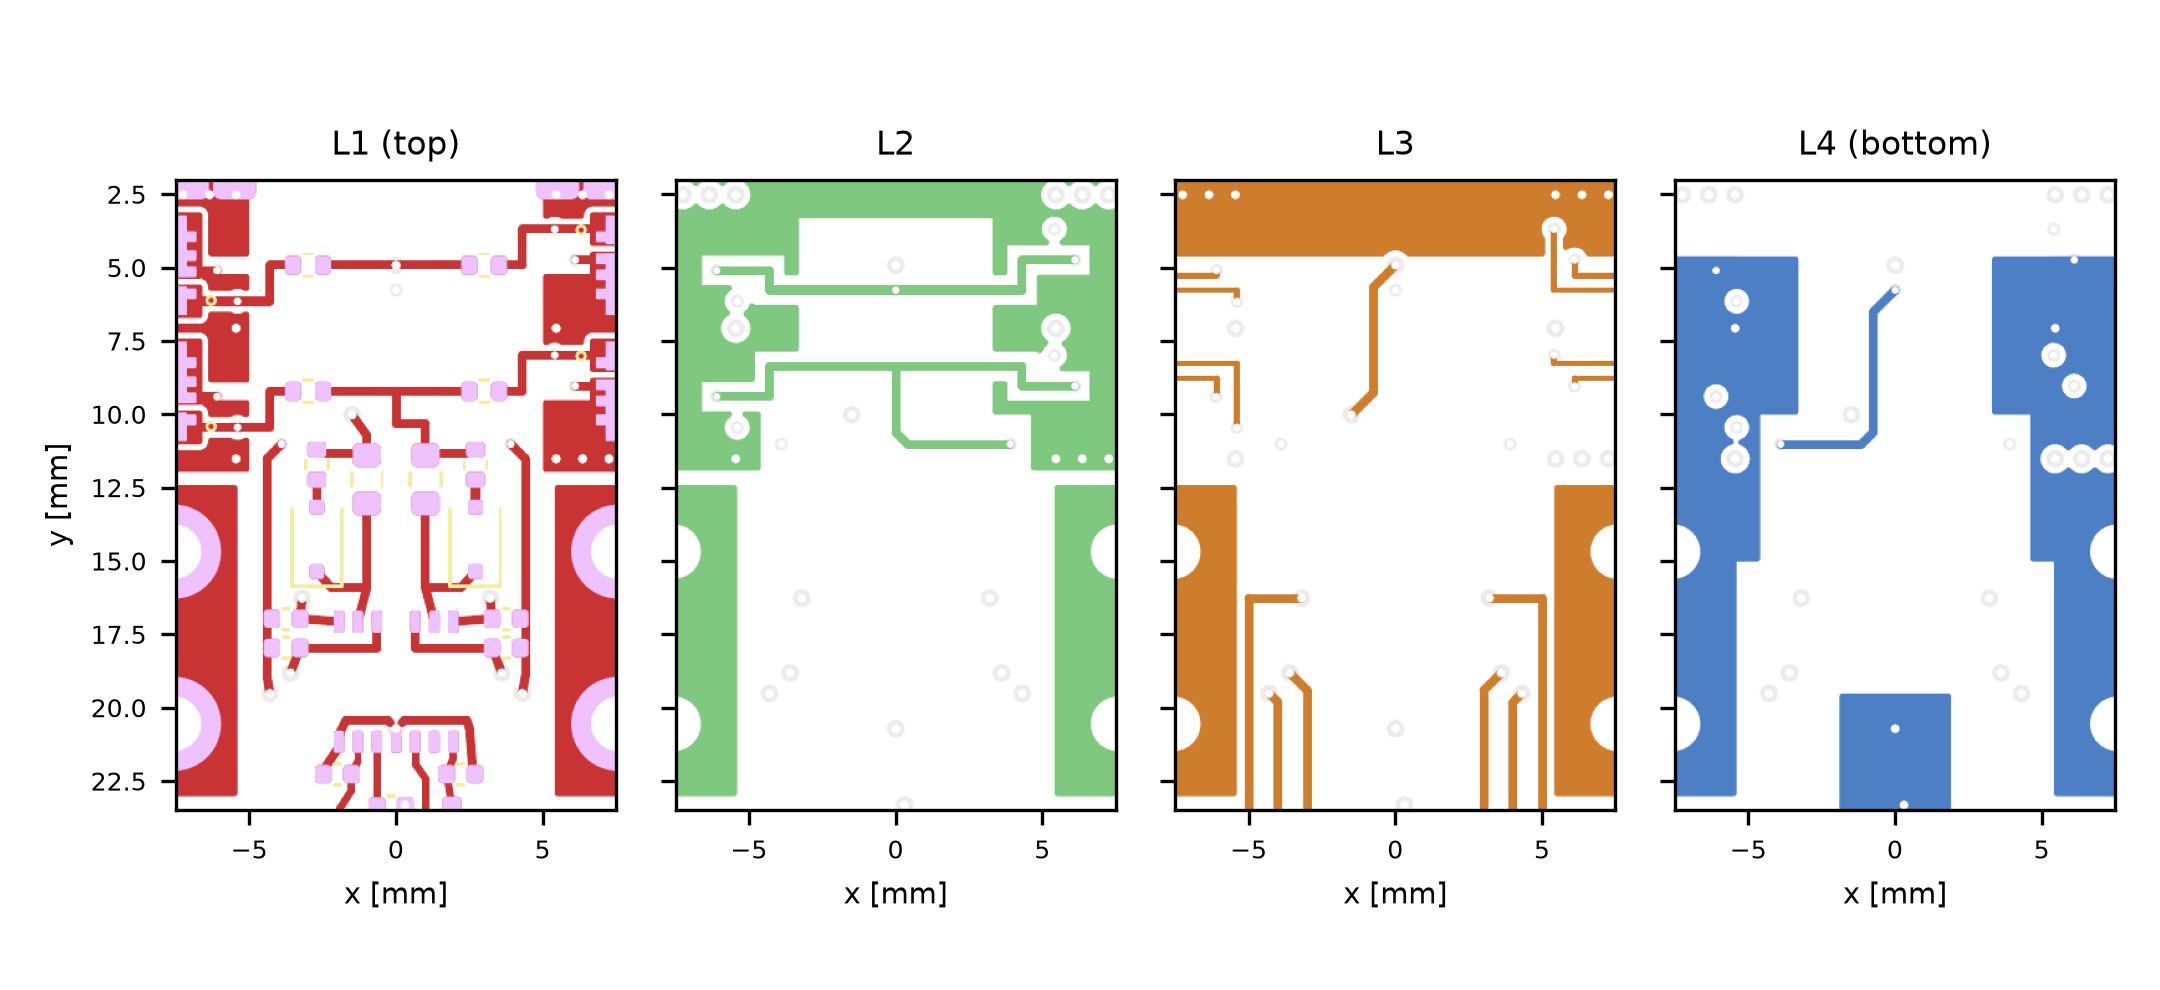
\includegraphics[width=\linewidth,height=0.62\textheight,keepaspectratio]{fig_corridor.png}
\small
\begin{itemize}
\item HS: trunk on L3, Kelvin return directly below on L4; LS: star on L1, Kelvin collector on L2
\item Kelvin collectors join on the symmetry line $\Rightarrow$ identical gate loops for both transistors
\end{itemize}
\end{frame}

\begin{frame}{Separate turn-on and turn-off paths}
\begin{columns}[T]
\column{0.5\textwidth}
\centering
\begin{circuitikz}[scale=0.8,transform shape]
\draw (0,0) node[left]{OUT} to[short,o-*] (1,0) to[R,l=$R_\mathrm{ON}$] (4,0) to[short,-*] (5,0);
\draw (1,0) -- (1,-1.5) to[D*,l_=$D$,invert] (2.6,-1.5) to[R,l_=$R_\mathrm{OFF}$] (4.6,-1.5) -- (5,-1.5) -- (5,0);
\draw (5,0) to[short] (5.6,0) node[right]{trunk / star};
\draw (5.6,0) -- (5.6,1) to[R,l=$R_{G,1}$] (8,1) node[right]{G$_1$};
\draw (5.6,0) -- (5.6,-1) to[R,l_=$R_{G,2}$] (8,-1) node[right]{G$_2$};
\draw (5.6,0) to[short,*-] (5.6,0);
\end{circuitikz}
\vspace{1ex}

\small $R_\mathrm{on,eff} = 2R_\mathrm{ON}+R_{G,i}$\\
$R_\mathrm{off,eff} \approx 2(R_\mathrm{ON}\parallel R_\mathrm{OFF})+R_{G,i}\;(+V_F)$
\column{0.48\textwidth}
\small
\begin{tabular}{@{}lll@{}}
\toprule
Part & default & per transistor \\
\midrule
$R_\mathrm{ON}$ (0603) & 0.75\,$\Omega$ & on: 2.0\,$\Omega$ \\
$R_\mathrm{OFF}$ (0402) & 0\,$\Omega$ & off: 0.5\,$\Omega$ + D \\
D PMEG3020EJ & SOD323F & \\
$R_{G,i}$ (0402) & 0.5\,$\Omega$ & \\
\bottomrule
\end{tabular}
\begin{itemize}
\item Peak gate current 3.1\,A (on) / 6.5\,A (off): within 4 / 8\,A
\item Same as the simulated 2\,$\Omega$ / 0\,$\Omega$ external
\item Values changeable by population
\item 10\,k$\Omega$ pull-down star $\rightarrow$ Kelvin per switch
\end{itemize}
\end{columns}
\end{frame}

\begin{frame}{Driver schematic (KiCad)}
\centering
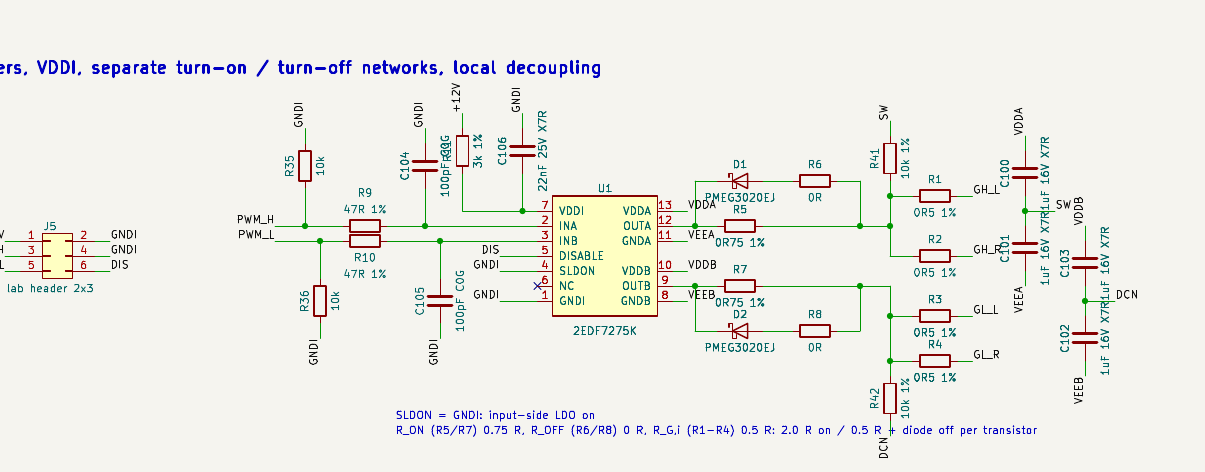
\includegraphics[width=\linewidth,height=0.8\textheight,keepaspectratio]{sch_driver.png}
\end{frame}

\begin{frame}{Isolated gate supplies}
\begin{columns}[T]
\column{0.5\textwidth}
\centering
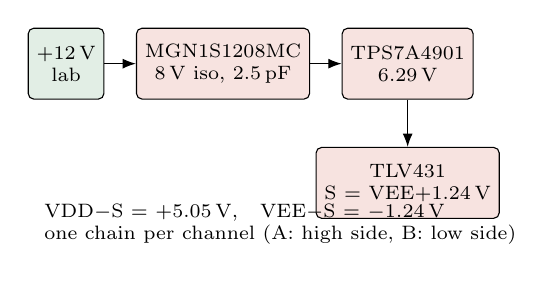
\begin{tikzpicture}[font=\scriptsize,node distance=4mm,
  b/.style={draw,rounded corners=2pt,minimum height=9mm,align=center,inner sep=3pt}]
\node[b,fill=pri!15] (p) {+12\,V\\lab};
\node[b,fill=hs!15,right=of p] (m) {MGN1S1208MC\\8\,V iso, 2.5\,pF};
\node[b,fill=hs!15,right=of m] (l) {TPS7A4901\\6.29\,V};
\node[b,fill=hs!15,below=6mm of l] (t) {TLV431\\S = VEE+1.24\,V};
\draw[-{Latex}] (p) -- (m); \draw[-{Latex}] (m) -- (l); \draw[-{Latex}] (l) -- (t);
\node[below=12mm of p,anchor=north west,align=left,xshift=-4mm] {VDD$-$S = +5.05\,V,\quad VEE$-$S = $-1.24$\,V\\one chain per channel (A: high side, B: low side)};
\end{tikzpicture}
\column{0.48\textwidth}
\small
\begin{itemize}
\item Two isolated supplies: HS reference = switch node, LS reference = DC$-$ (floats up to 1.2\,kV in the stack)
\item TPS7A4901 replaces LP2951: LP2951 has no VSSOP and its legacy chip needs ESR $\geq$\,30\,m$\Omega$
\item $V_\mathrm{OUT} = 1.185\,\mathrm{V}\,(1+102\,\mathrm{k}/23.7\,\mathrm{k})$; stable with ceramics $\geq$\,2.2\,\textmu F
\item TLV431 stable: $>$\,5\,\textmu F on S$-$VEE (unstable band 0.02--0.8\,\textmu F)
\item Budget per channel at 50\,kHz: 65\,nC, 7.6\,mA, 61\,mW
\end{itemize}
\end{columns}
\end{frame}

\begin{frame}{Supply schematic (KiCad)}
\centering
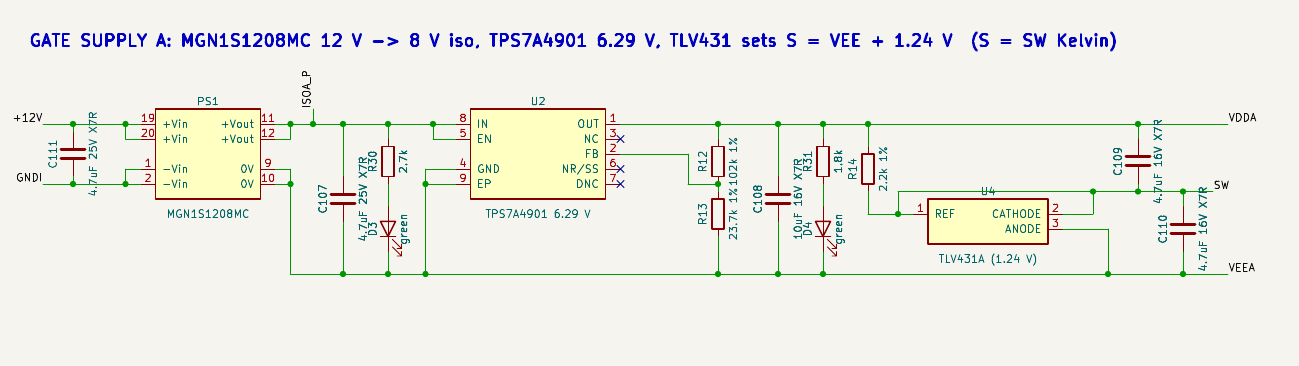
\includegraphics[width=\linewidth,height=0.8\textheight,keepaspectratio]{sch_supply.png}
\end{frame}

\begin{frame}{Isolation domains}
\begin{columns}[T]
\column{0.5\textwidth}
\small
\begin{tabular}{@{}lrr@{}}
\toprule
Domains & outer & inner \\
\midrule
DC$+$ -- switch node & 0.20 & 0.65 \\
DC$+$ -- DC$-$ & 0.70 & 1.07 \\
HS -- LS & 0.20 & 0.40 \\
HS -- primary & 1.37 & 1.08 \\
LS -- primary & 1.50 & 0.75 \\
\bottomrule
\end{tabular}
{\scriptsize minimum copper spacing [mm] on the routed board}
\column{0.48\textwidth}
\small
\begin{itemize}
\item Power domains $\leq$\,100\,V: 0.2\,mm under mask
\item Primary side separated functionally (lab board)
\item In the 1200\,V stack: PWM via fibre / reinforced isolator and isolated 12\,V at the controller side; 2EDF7275K is functional only
\end{itemize}
\end{columns}
\end{frame}

%==================================================================== 11
\section{Measurements and bring-up}
\begin{frame}{Double-pulse test: measurement landings}
\begin{columns}[T]
\column{0.55\textwidth}
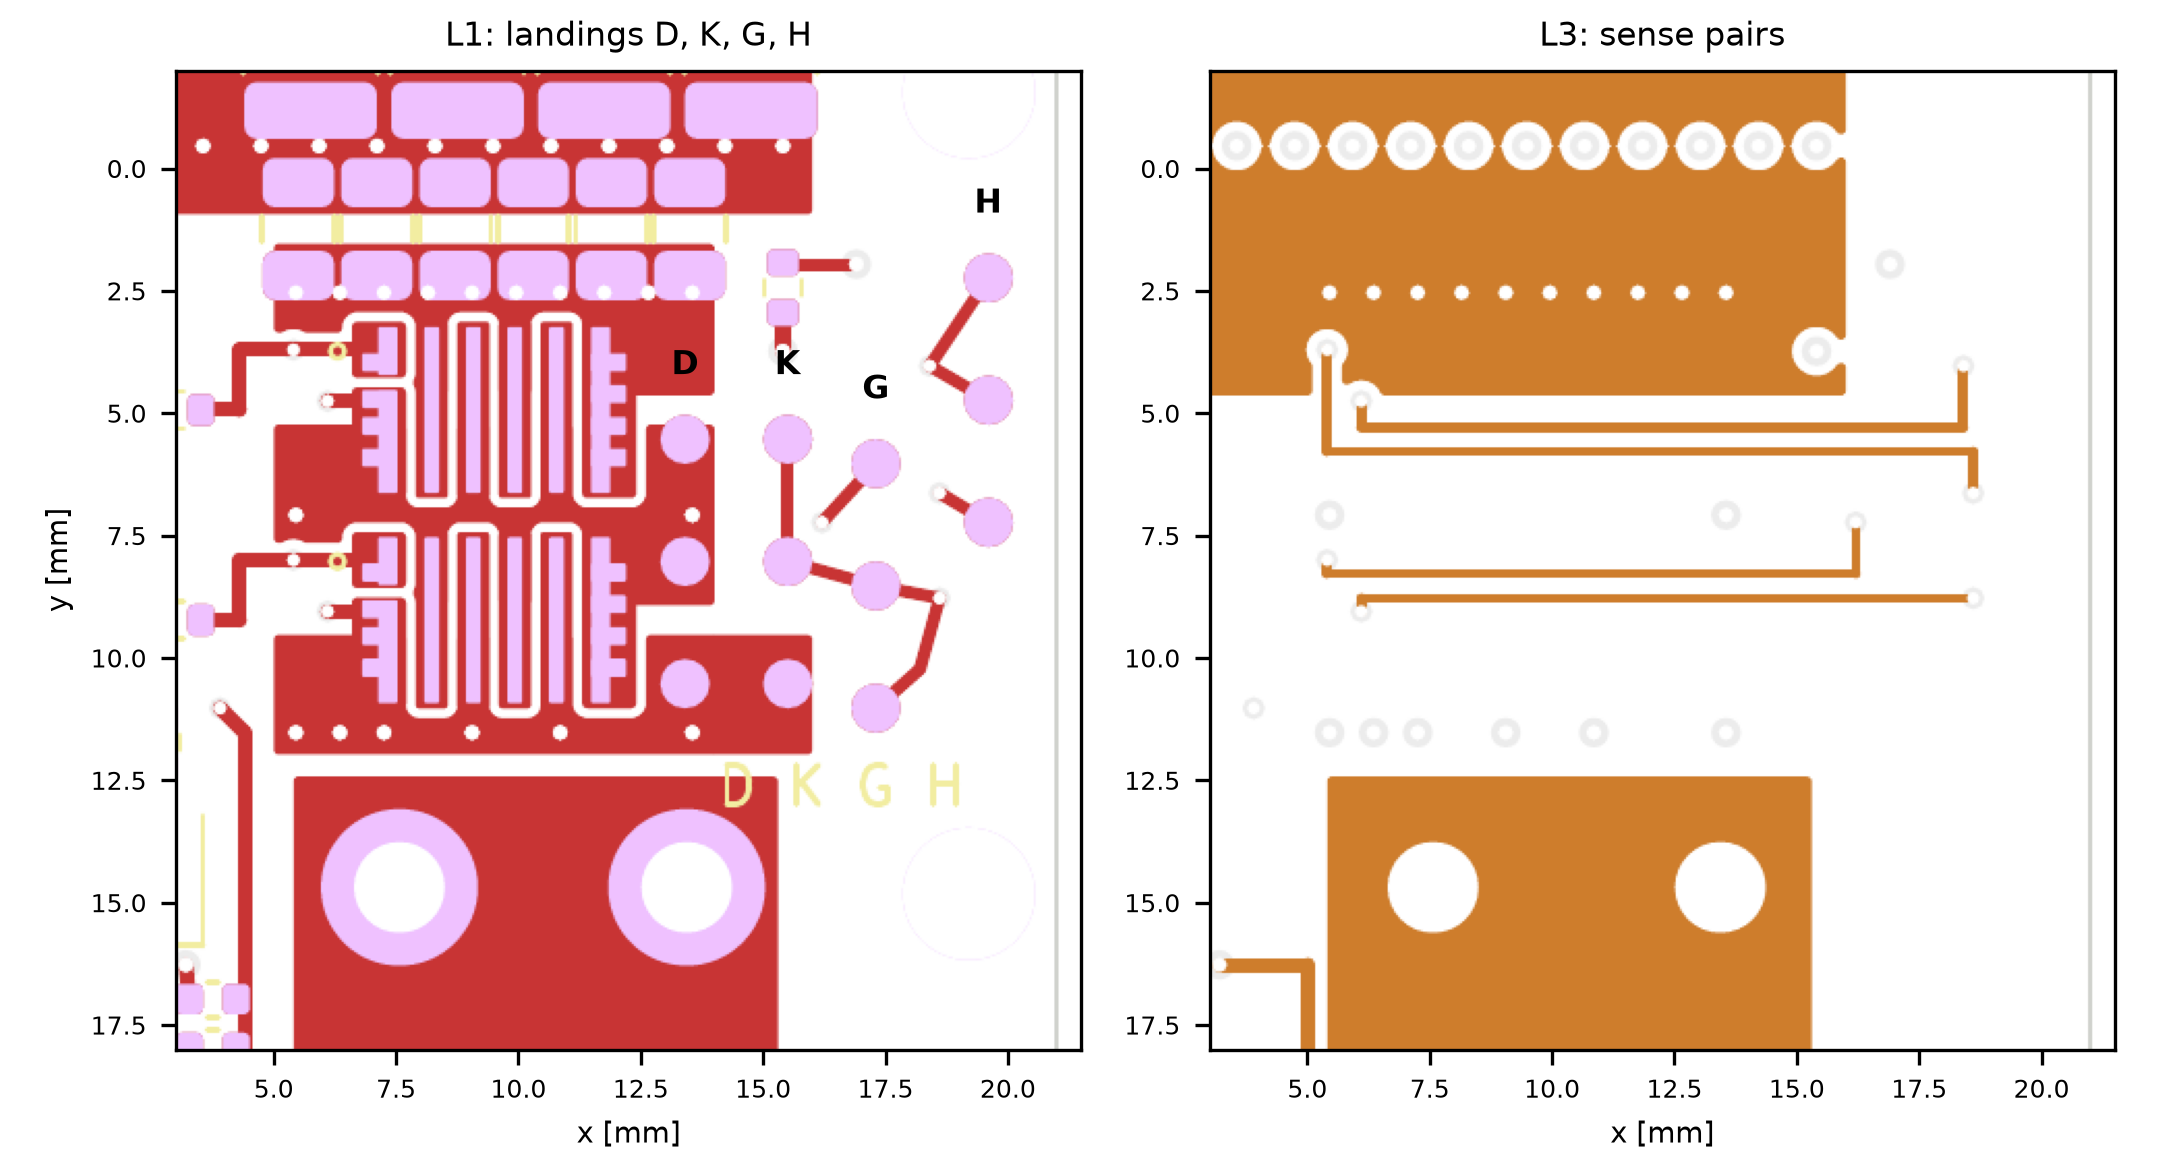
\includegraphics[width=\linewidth]{fig_landings.png}
\column{0.43\textwidth}
\small
\begin{itemize}
\item Probe pads only, outside the commutation loop; spring ground at 2.5 and 5.0\,mm
\item \textbf{D}: $V_{DS}$ of Q3 / Q4 at the package
\item \textbf{K}: $v_{KS}$ = Kelvin vs power-source copper
\item \textbf{G}: $V_{GS}$ of Q3 / Q4 (sense pairs on L3)
\item \textbf{H}: $V_{GS}$ of Q1 / Q2 (isolated probe)
\item Inductor current: Rogowski / Pearson off the board
\end{itemize}
\end{columns}
\end{frame}

\begin{frame}{$E_\mathrm{on}$, $E_\mathrm{off}$ and per-transistor current}
\small
\begin{itemize}
\item $E = \int v_{DS}\, i_D\, dt$; $E_\mathrm{off}$ with $i_D = I_L$; $E_\mathrm{on}$ with $I_L$ plus the high-side output charge $Q_\mathrm{OSS}V_\mathrm{DC}$
\item Deskew $<$\,50\,ps: 100\,ps at 50\,V/ns and 100\,A $\approx$ 0.75\,\textmu J error ($\approx$\,8\,\% of $E_\mathrm{on}$)
\item Per-transistor current without a shunt (no extra loop inductance):
\[ v_{KS} = L_s\,\frac{di_D}{dt} + R_s i_D \quad\Rightarrow\quad \Delta i_D(t) \approx \frac{1}{L_s}\int v_{KS}\,dt \]
$L_s \approx 0.03$\,nH: $\approx$\,0.5\,V at 17\,A/ns; scale with $i_3+i_4 = I_L$, ratio gives the dynamic sharing
\item Same principle as stray-inductance di/dt sensing in SiC short-circuit protection (Sun, CPES 2019; Xue et al., TPEL 2020)
\item Rogowski holes in the cells: not possible without opening the L1/L2 loop; coil bandwidth (20--50\,MHz) too low for 2--3\,ns edges
\end{itemize}
\end{frame}

\begin{frame}{Bring-up: test points, LEDs, protection}
\begin{columns}[T]
\column{0.55\textwidth}
\scriptsize
\begin{tabular}{@{}lll@{}}
\toprule
Item & nets & expected \\
\midrule
TP15, D7 & +12\,V & 12\,V present \\
TP9/12, D3/5 & ISO / VEE & MGN1 output 8--10\,V \\
TP10/13, D4/6 & VDD / VEE & 6.29\,V \\
TP11/14 & S / VEE & 1.24\,V \\
TP16, D8 (red) & DC link & charged; 100\,k bleeder \\
R35/R36 & PWM & 10\,k pull-downs \\
R41/R42 & star--Kelvin & 10\,k gate pull-downs \\
J7 & +12\,V & fan \\
\bottomrule
\end{tabular}
\column{0.43\textwidth}
\small
\textbf{Power-up order}
\begin{enumerate}\footnotesize
\item 12\,V (current limit), LEDs on, TP values
\item PWM without DC link: driver outputs on R5/R7, gates on R1--R4
\item DC link 12 $\rightarrow$ 24 $\rightarrow$ 48 $\rightarrow$ 75\,V, double-pulse test
\item Heatsink, continuous operation
\end{enumerate}
\footnotesize Power down in reverse: DC link first, then 12\,V.
\end{columns}
\end{frame}

\begin{frame}{Cooling for the load test}
\begin{columns}[T]
\column{0.55\textwidth}
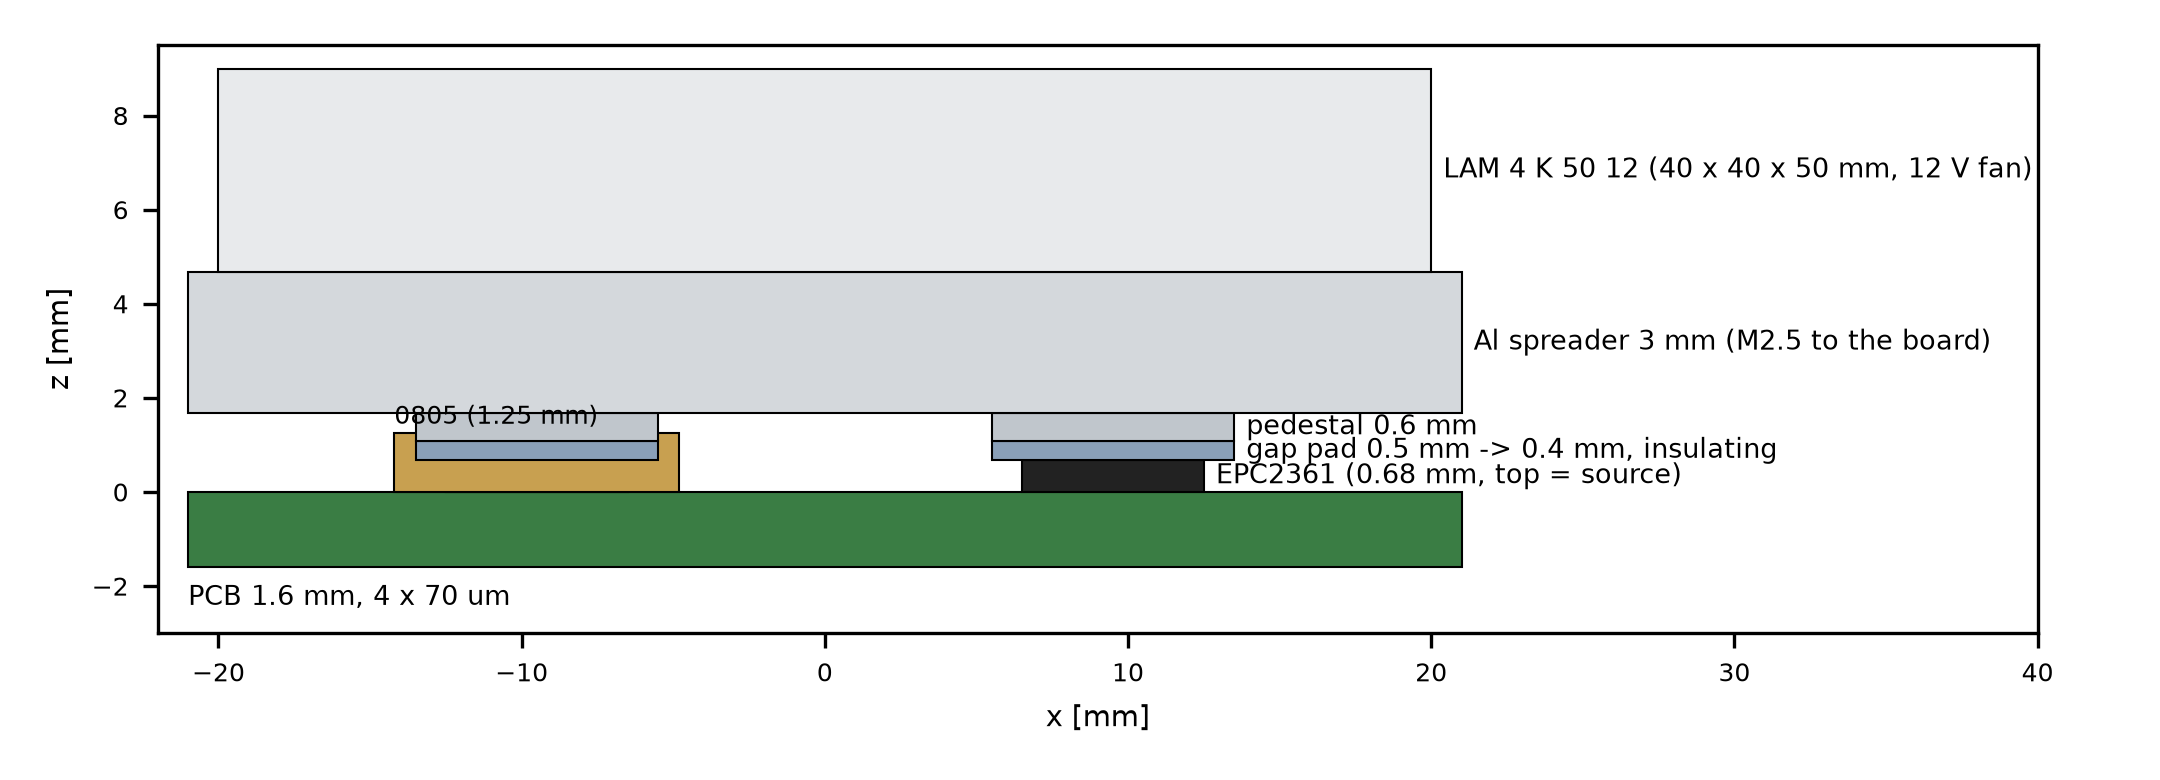
\includegraphics[width=\linewidth]{fig_heatsink.png}
\column{0.43\textwidth}
\small
\begin{itemize}
\item Fischer LAM 4 K 50 12 (0.65\,K/W, 12\,V fan from J7), off the shelf
\item Al spreader 42\,$\times$\,14\,$\times$\,3\,mm (workshop part), 4\,$\times$ M2.5
\item Insulating gap pad 0.5\,mm, $\geq$\,5\,W/mK: 5.3\,K/W per transistor (dominant)
\item $T_j \approx 57\,^\circ$C (40\,$^\circ$C ambient); flat plate + 1\,mm pad: $\approx$\,70\,$^\circ$C
\item Next step: AlN insulator ($\approx$\,1\,K/W per transistor)
\end{itemize}
\end{columns}
\end{frame}

\begin{frame}{Power-stage schematic (KiCad)}
\centering
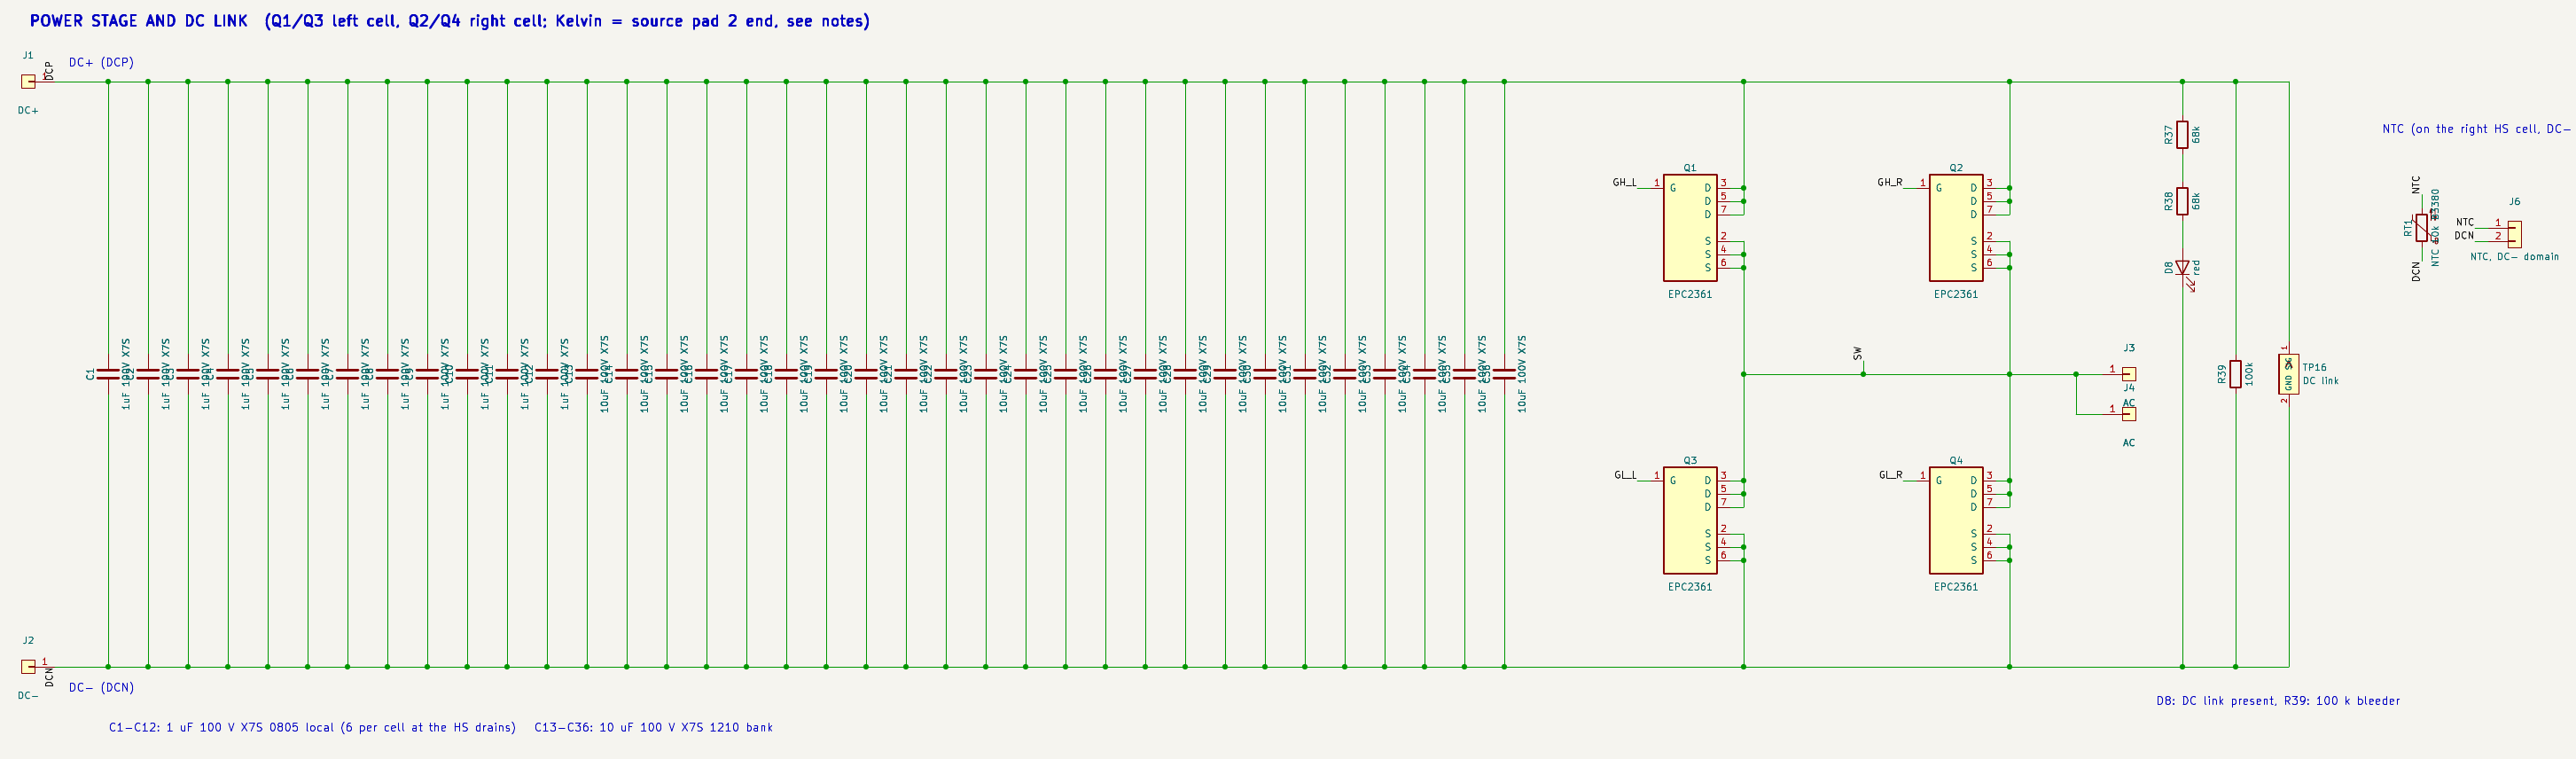
\includegraphics[width=\linewidth,height=0.8\textheight,keepaspectratio]{sch_power.png}
\end{frame}

%==================================================================== 12
\section{Status and next steps}
\begin{frame}{Verification status}
\small
\begin{tabularx}{\linewidth}{@{}lX@{}}
\toprule
Done & DRC 0 violations / 0 unconnected; wired schematic = PCB netlist (37 nets); 3D models for all parts, STEP export; Gerber, drill, pick-and-place, BOM (35 lines, 107 parts + mechanics); datasheet checks: TPS7A4901 pins/stability, TLV431 pinout and stability, PMEG3020EJ \\
Prepared & Q3D re-extraction of the routed copper (\texttt{run\_bb\_q3d\_fab.cmd}); needs the KTH licence (campus / VPN) \\
Open & Q3D result vs 0.374\,nH design value; gap-pad part and spreader drawing; fab-house review of 0.2\,mm gaps; isolation concept for the 1200\,V stack \\
\bottomrule
\end{tabularx}
\end{frame}

\begin{frame}{Next steps}
\begin{enumerate}
\item Re-extract the routed board in Q3D, update loop and gate-loop values
\item Order Rev A, assemble, bring-up (12\,V, PWM, then DC link)
\item Double-pulse test at 12--75\,V: $E_\mathrm{on}$, $E_\mathrm{off}$, gate bump, sharing (D, G, K, H landings)
\item Continuous operation with the fan heatsink; thermal camera
\item Compare with LTspice / Q3D; decide 75\,V vs 60\,V submodules
\item Rev B: cell interconnect with laminated tabs, AlN interface, integration form factor (36\,mm pitch)
\end{enumerate}
\end{frame}

\begin{frame}[standout]
Thank you\\[1ex]
\small Questions?
\end{frame}

\end{document}
